\section{Numerical Simulation}

\frame{\sectionpage}

\begin{frame}{Alternative Knockoff Statistics}
    \small
    For a statistic $\mathbf{T}$ for each original and knockoff variable $$ \mathbf{T} \overset{\Delta}{=} (\mathbf{Z},\tilde{\mathbf{Z}}) = (Z_1,\cdots,Z_p,\tilde{Z}_1,\cdots,\tilde{Z}_p) = t\left\{ (\mathbf{X},\tilde{\mathbf{X}}), \mathbf{y}\right\} $$
    set $$W_j = f_j(Z_j,\tilde{Z}_j)$$ where $f_j$ is any \textcolor{glaucous!65!white}{\textbf{antisymmetric}} function (\underline{$f(v,u)=-f(u,v)$}) to achieve the flip sign condition.

    \vspace*{5pt}
    \normalsize
    \begin{itemize}
        \item<2-> \textit{\underline{Alternative}} knockoff statistics 
        \item<2-> \textit{\underline{Bayesian}} knockoff statistics
    \end{itemize}
\end{frame}

\begin{frame}{Alternative Knockoff Statistics: LCD vs LSM}
    
    {\footnotesize \begin{align*}
        W_j &= Z_j -\tilde{Z}_j = \lvert \hat{b}_j(\lambda) \rvert - \lvert \hat{b}_{j+p}(\lambda) \rvert & \text{where } &\hat{b} = \arg\min_{b\in\mathbb{R}^{2p}}\frac{1}{2}\lVert y - (\mathbf{X},\tilde{\mathbf{X}})b \rVert^2_2 + \lambda \lVert b \rVert _1 & (\mathrm{LCD})\\
        W_j &=\mathrm{sgn}(\lvert Z_j \rvert-\lvert \tilde{Z}_j \rvert)\max\left\{ \lvert Z_j \rvert,\lvert \tilde{Z}_j \rvert \right\} & \text{where } &Z_j = \sup \left\{ \lambda:\hat{b}_j(\lambda)\neq 0 \right\} & (\mathrm{LSM})
    \end{align*}}

    \uncover<2->{\begin{figure}\label{fig:LSM_vs_LCD}
        \centering
        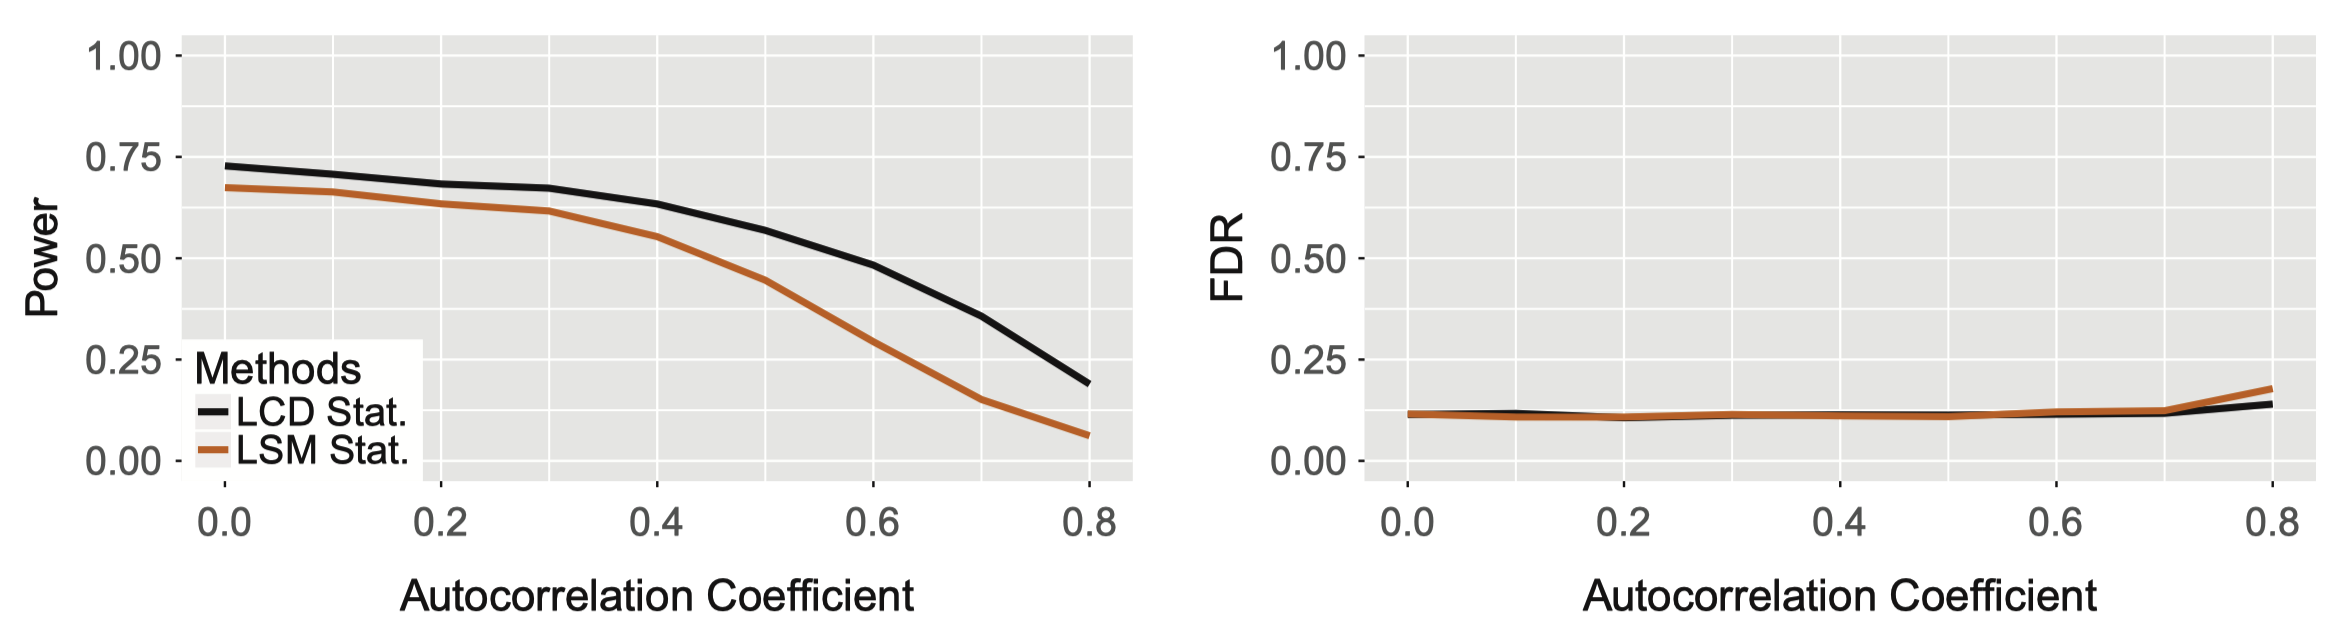
\includegraphics[width = 0.95 \textwidth]{images/lsm_vs_lcd.png}
    \end{figure}}
    \vspace*{5pt}
\end{frame}

\begin{frame}{Alternative Knockoff Statistics: LCD vs BVS}
    BVS: $Z_j-\tilde{Z}_j$ where $Z_j$ and $\tilde{Z}_j$ are the posterior probabilities that the $j$th original and knockoff coefficients are \textit{\underline{non-zero}} respectively.
    \begin{figure}\label{fig:BVS_vs_LCD}
        \centering
        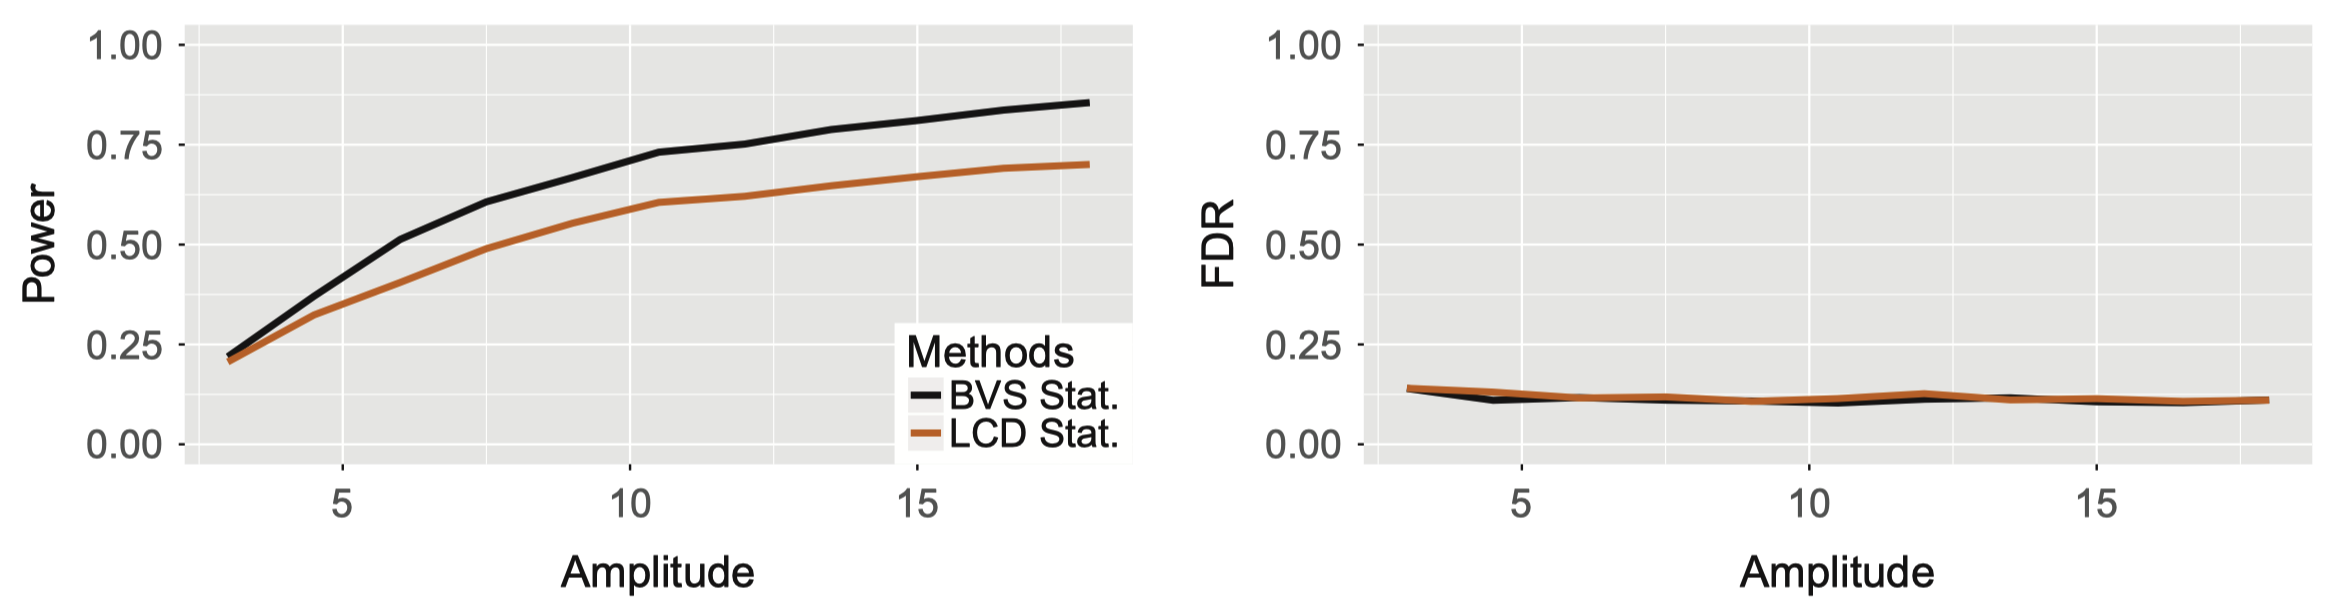
\includegraphics[width = 0.95 \textwidth]{images/bvs_vs_lcd.png}
    \end{figure}
\end{frame}

\begin{frame}{Alternative Procedures: $BH$ conditional randomization test}

    {\footnotesize
    \begin{itemize}
        \item for $(\mathbf{X},\mathbf{y})$ and $k=1,\cdots,K$, simulate $\mathbf{X}^{(k)}$ by simulating the $j$th column of $\mathbf{X}$ from $\mathcal{L}(\mathbf{X}_j\mid \mathbf{X}_{-j})$
        \item calculate $p-$value as $ P_j = \frac{1}{K+1}\left[ 1+\sum^K_{k=1}\mathbf{1}_{T_j(\mathbf{X}^{(k)},\mathbf{y})\geq T_j(\mathbf{X},\mathbf{y})} \right] $
    \end{itemize}   }
    \vspace*{-10pt}
    \begin{figure}\label{fig:procedure1}
        \centering
        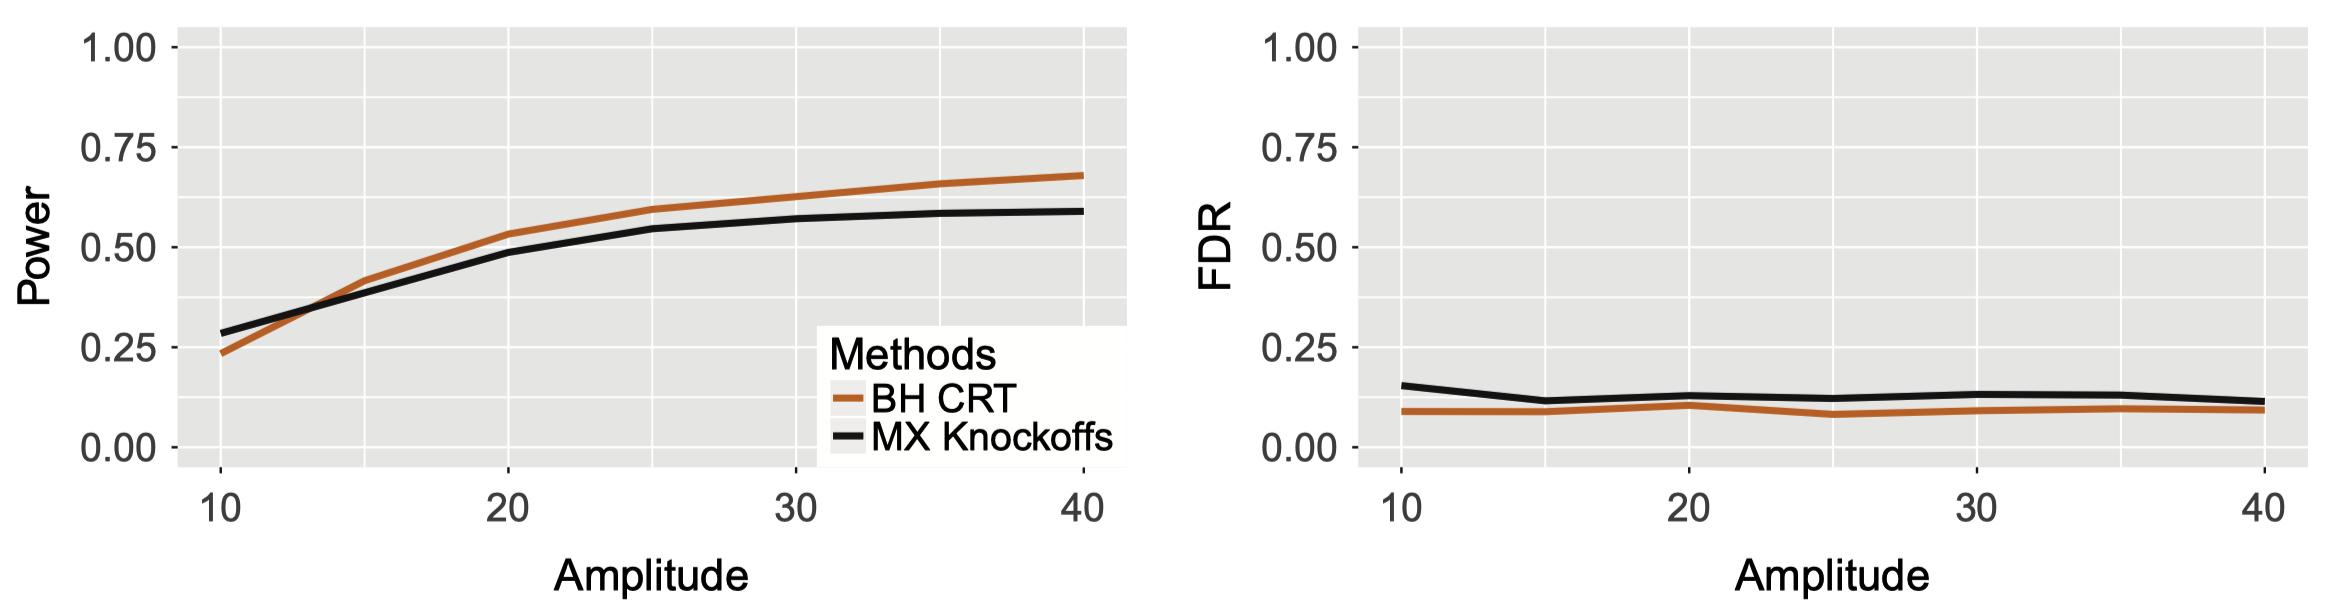
\includegraphics[width = 0.95 \textwidth]{images/altproced_1.png}
    \end{figure}
\vspace*{-5pt}
    \hfill $BH$ CRT is \textit{very} computationally costly (by 5000 times)!
\end{frame}

\begin{frame}{Alternative Procedures: Independent Covariates + Gaussian}

    {\footnotesize
    \begin{itemize}
        \item $FX$ knockoff: only applicable when $n\gg p$
        \item $BH$ applied to asymptotic GLM $p$-values: only applicable when $n\gg p$
        \item $BH$ applied to marginal test $p-$values: value for testing hypothesis of \textit{\underline{marginal}} distribution of $X_j$
    \end{itemize}   }
    \uncover<2->{\begin{columns}[T]
        \begin{column}{0.45\textwidth}
            \begin{figure}\label{fig:procedure2_a}
                \centering
                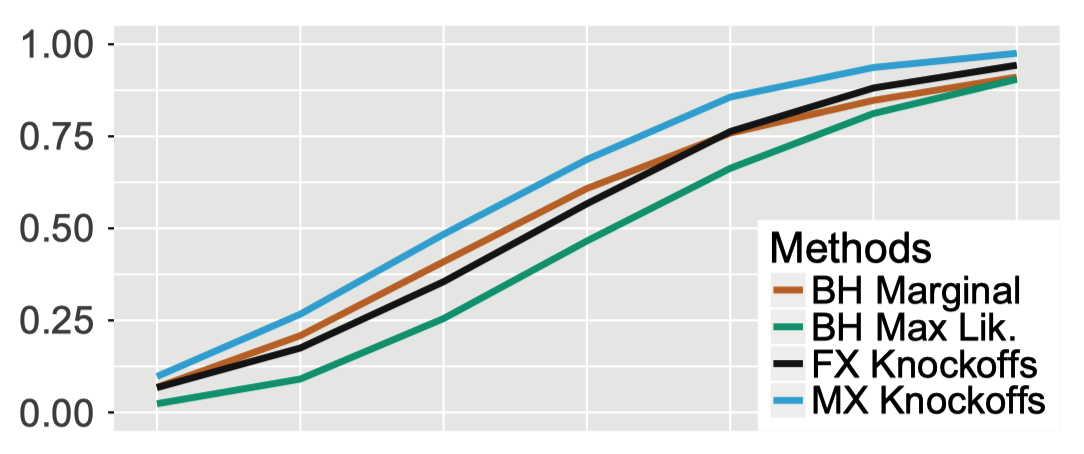
\includegraphics[width = \textwidth]{images/altproced_2_a.png}
            \end{figure}
            $$ n=3000,p=1000 $$
        \end{column}

        \begin{column}{0.45\textwidth}
            \begin{figure}\label{fig:procedure2_b}
                \centering
                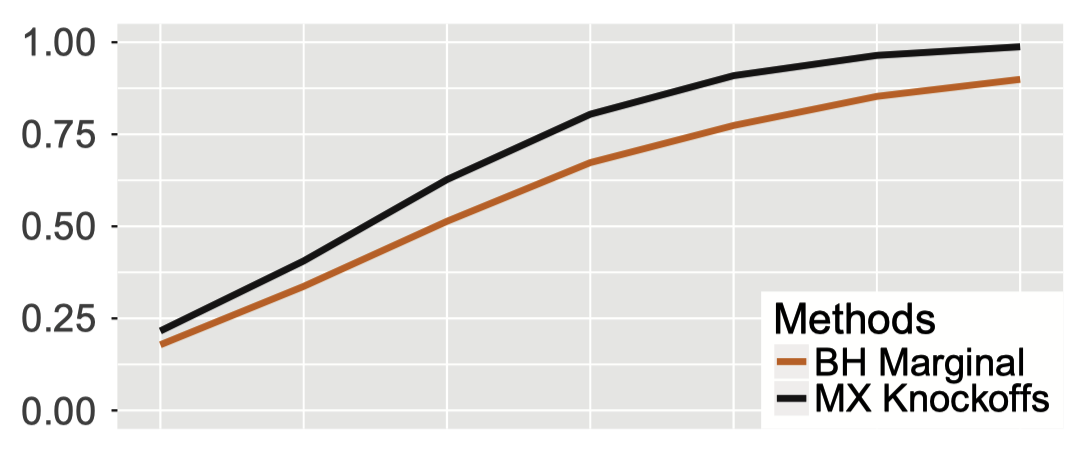
\includegraphics[width = \textwidth]{images/altproced_2_b.png}
            \end{figure}
            $$ n=3000,p=6000 $$
        \end{column}
    \end{columns}}
\end{frame}

\begin{frame}{Alternative Procedures: Independent Covariates + Binomial}
    \vspace*{-20pt}
    \uncover{\begin{columns}[T]
        \begin{column}{0.45\textwidth}
            \begin{figure}\label{fig:procedure3_a}
                \centering
                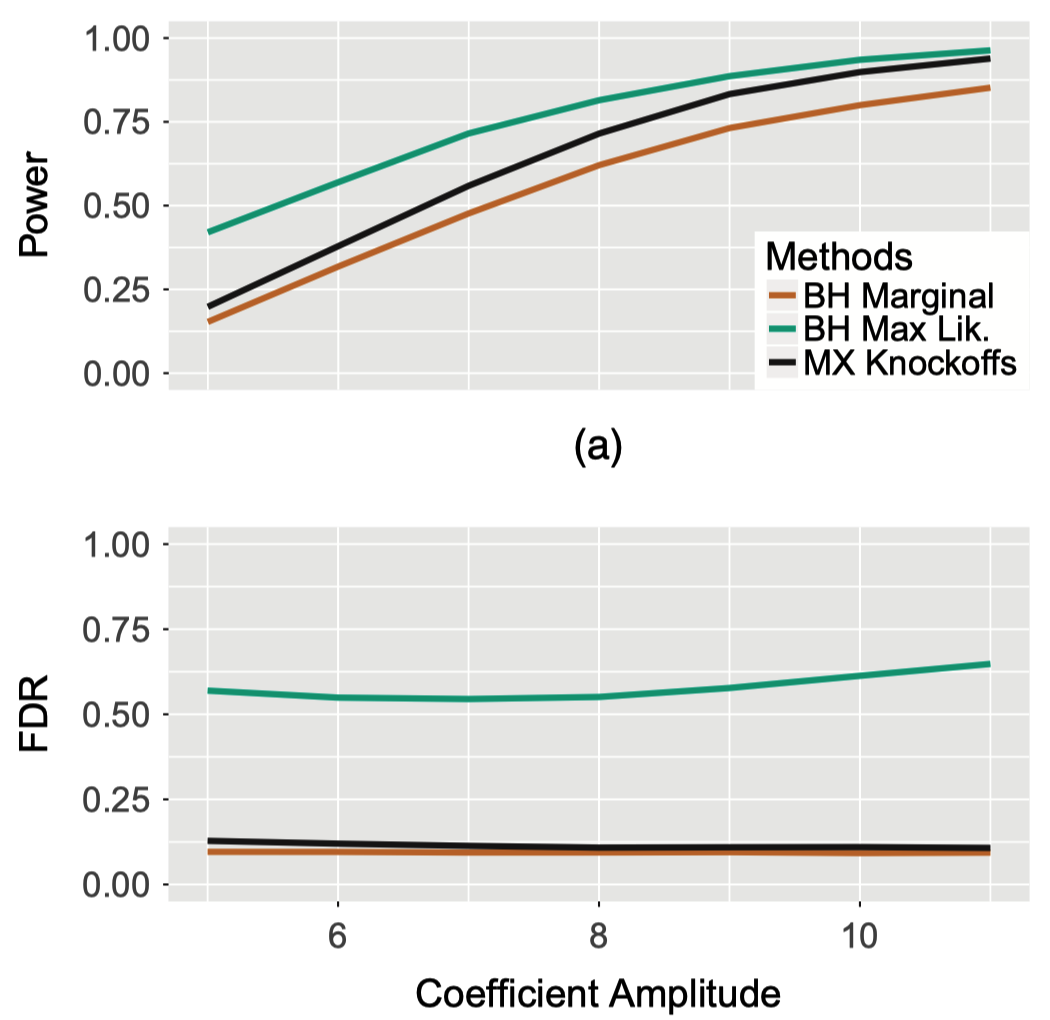
\includegraphics[height = 0.7\textheight]{images/altproced_3_a.png}
            \end{figure}
            \vspace*{-10pt}
            $$ n=3000,p=1000 $$
        \end{column}

        \begin{column}{0.45\textwidth}
            \begin{figure}\label{fig:procedure3_b}
                \centering
                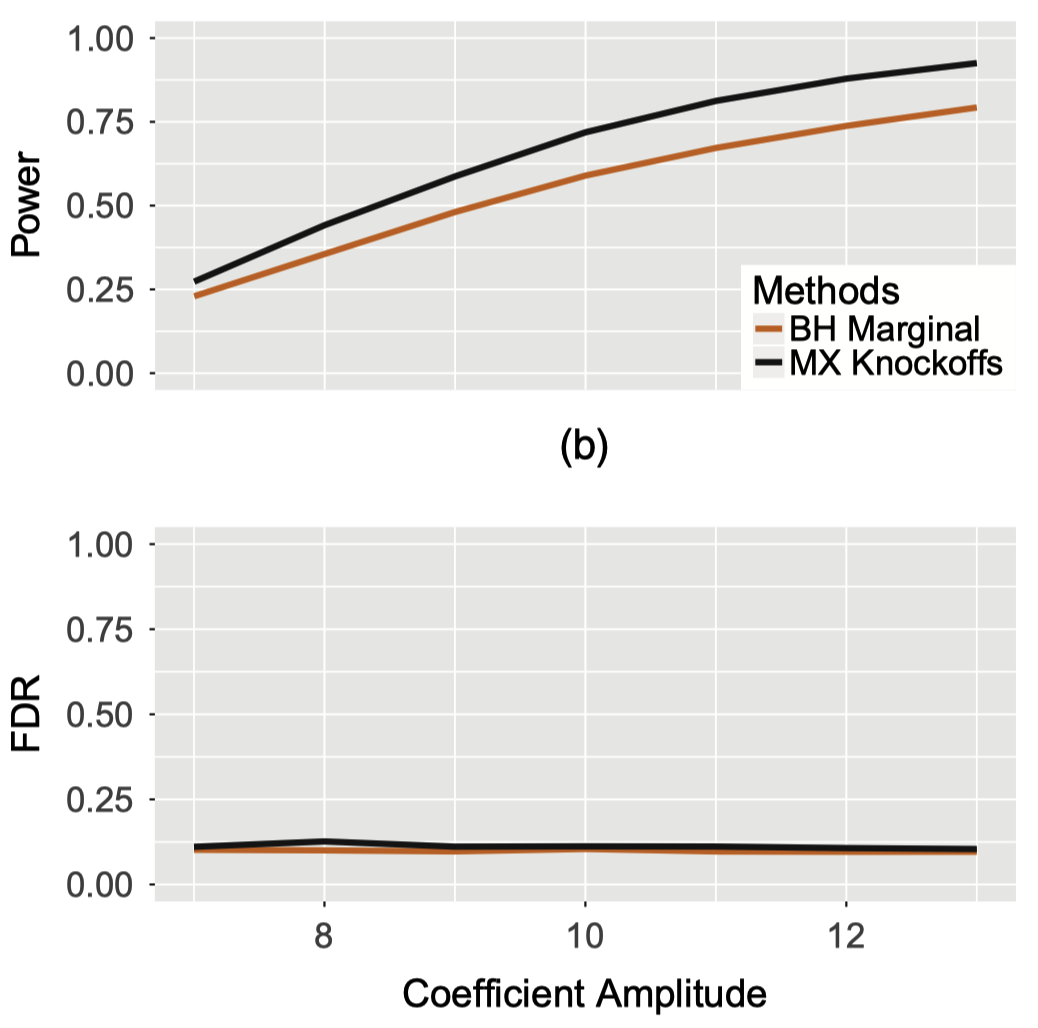
\includegraphics[height = 0.7\textheight]{images/altproced_3_b.png}
            \end{figure}
            \vspace*{-10pt}
            $$ n=3000,p=6000 $$
        \end{column}
    \end{columns}}
\end{frame}

\begin{frame}{Alternative Procedures: AR(1) Covariates}
    \vspace*{-20pt}
    \uncover{\begin{columns}[T]
        \begin{column}{0.45\textwidth}
            \begin{figure}\label{fig:procedure4_a}
                \centering
                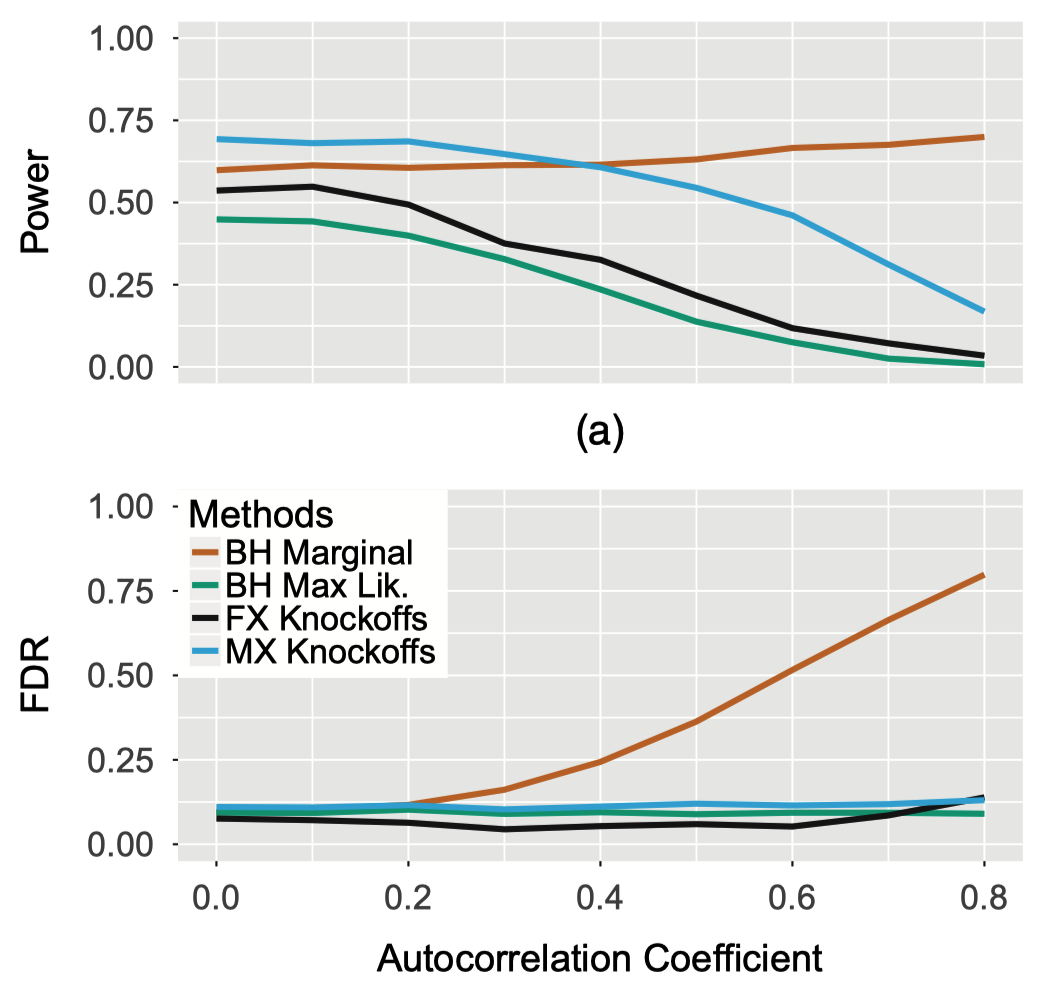
\includegraphics[height = 0.7\textheight]{images/altproced_4_a.png}
            \end{figure}
            \vspace*{-10pt}
            $$ n=3000,p=1000\text{; Gaussian} $$
        \end{column}

        \begin{column}{0.45\textwidth}
            \begin{figure}\label{fig:procedure4_b}
                \centering
                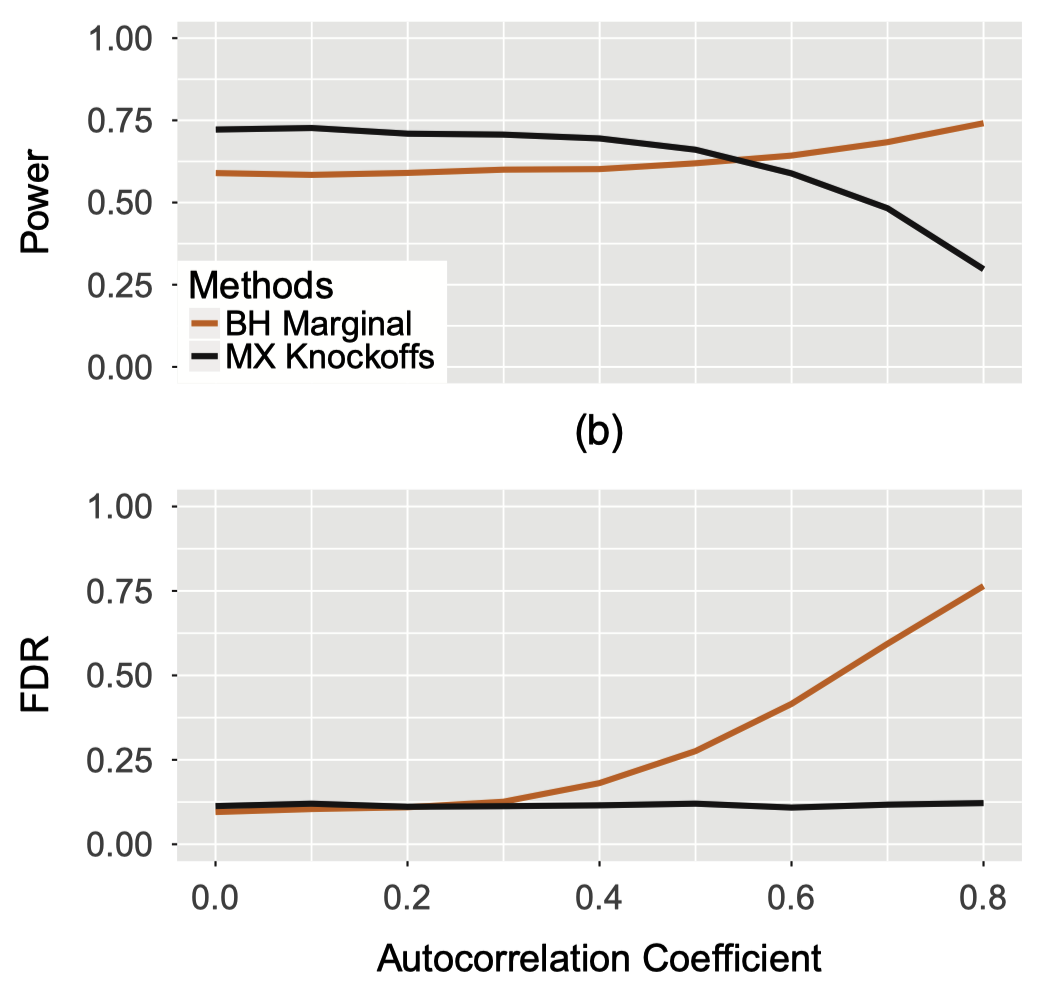
\includegraphics[height = 0.7\textheight]{images/altproced_4_b.png}
            \end{figure}
            \vspace*{-10pt}
            $$ n=3000,p=6000\text{; Binomial} $$
        \end{column}
    \end{columns}}
\end{frame}

\begin{frame}{Robustness: Overfitting Error}
    \begin{figure}\label{fig:robust1}
        \centering
        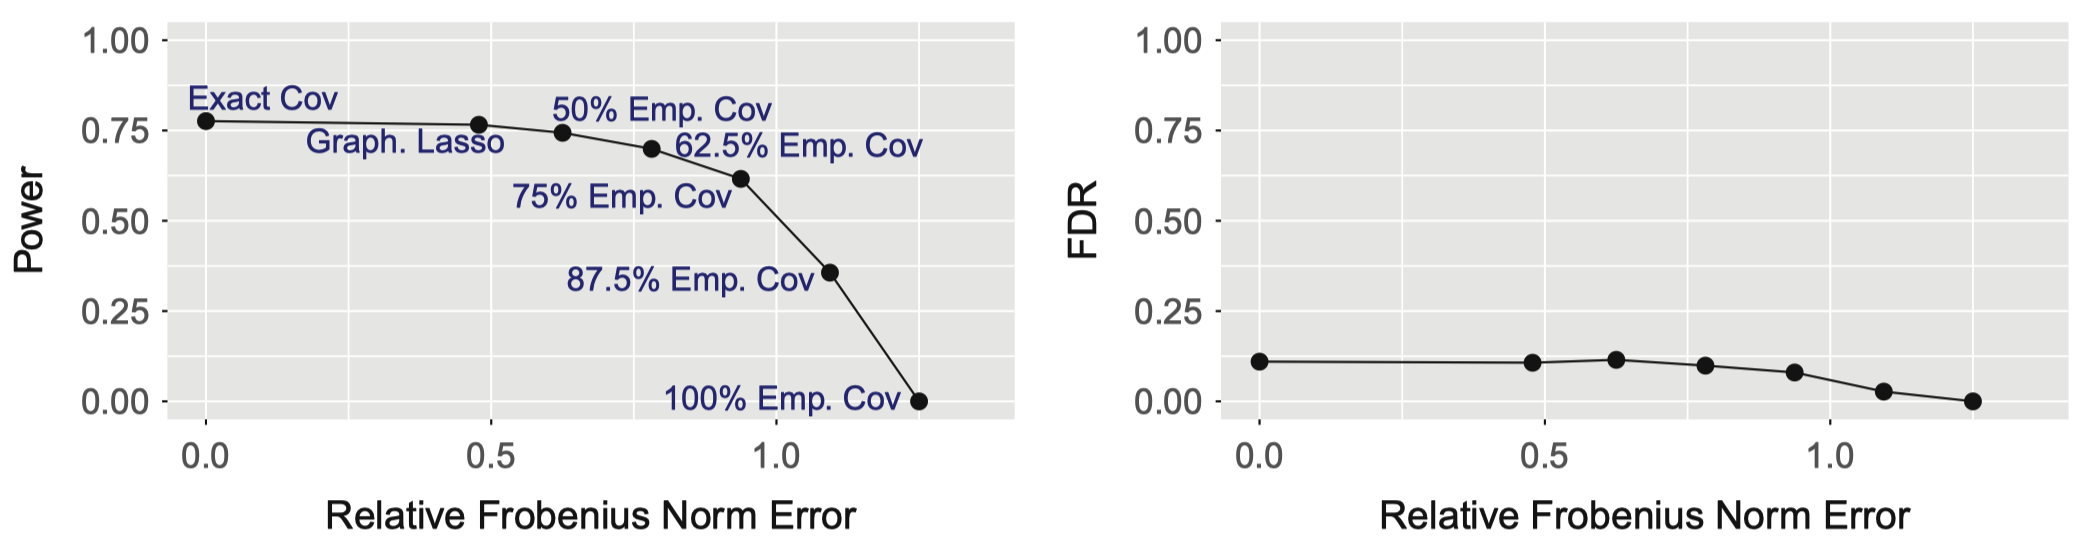
\includegraphics[width = 0.95 \textwidth]{images/robust1.png}
    \end{figure}
\end{frame}

\begin{frame}{Robustness: coefficient Amplitude}
    \begin{figure}\label{fig:robust2}
        \centering
        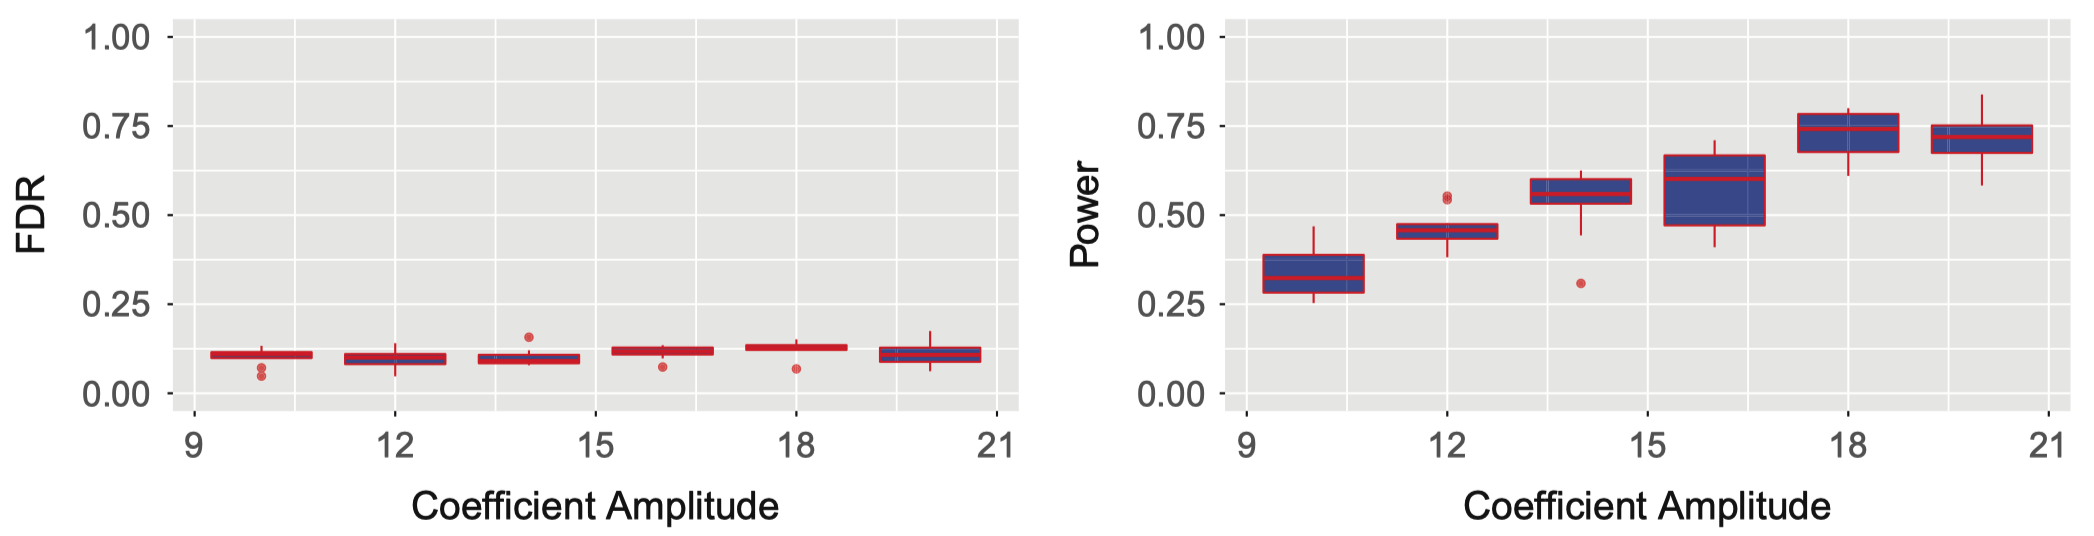
\includegraphics[width = 0.95 \textwidth]{images/robust2.png}
    \end{figure}
\end{frame}

\begin{frame}{Robustness: Shrinkage Multiplier}
    \begin{figure}\label{fig:robust3}
        \centering
        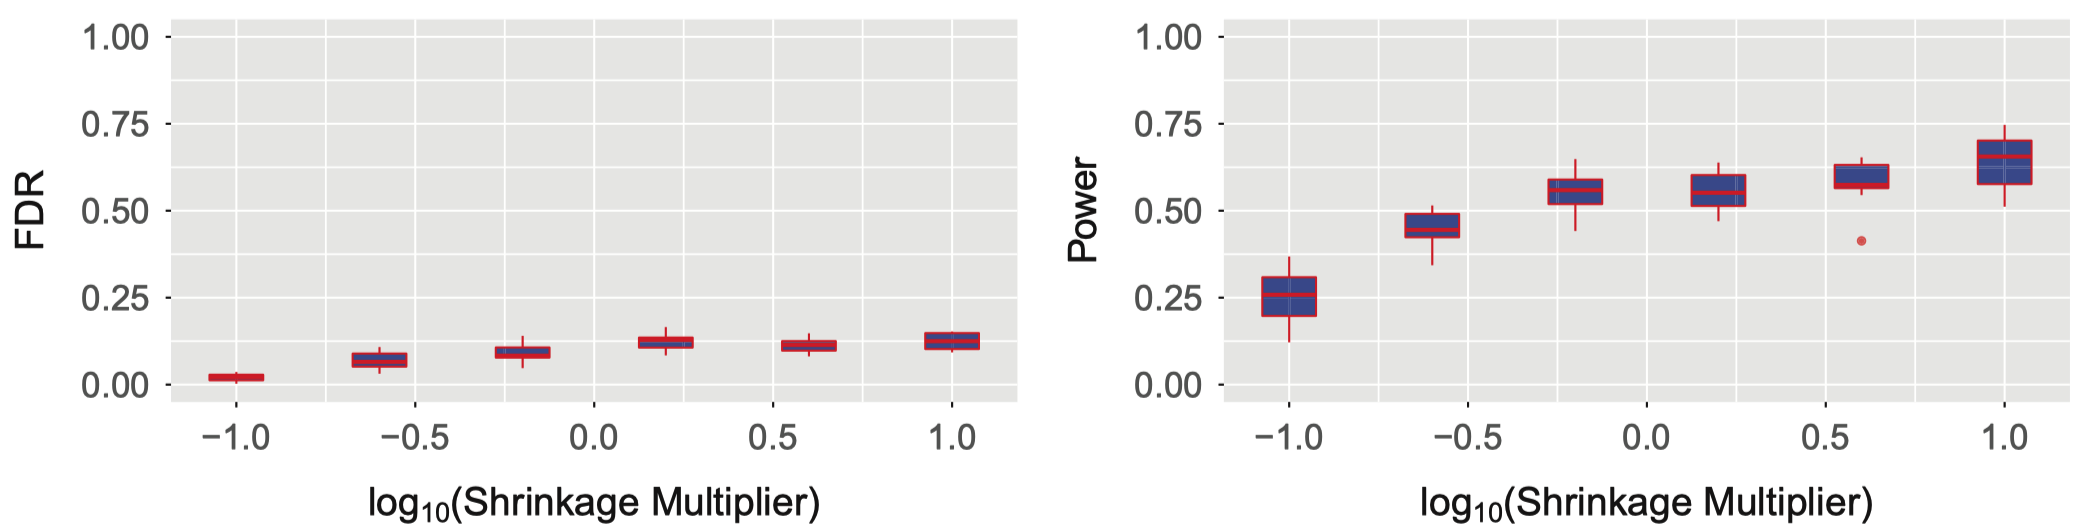
\includegraphics[width = 0.95 \textwidth]{images/robust3.png}
    \end{figure}
\end{frame}